\chapter{Практические задания}
\section{Задание}
\vspace{-0.7cm}
Используя хвостовую рекурсию, разработать эффективную программу,
(комментируя назначение аргументов), позволяющую:
\begin{enumerate}
	\item Сформировать список из элементов числового списка, больших заданного
	значения;
	\item Сформировать список из элементов, стоящих на нечетных позициях исходного
	списка (нумерация от 0);
	\item Удалить заданный элемент из списка (один или все вхождения);
	\item Преобразовать список в множество (можно использовать ранее разработанные
	процедуры).
\end{enumerate}
Убедиться в правильности результатов. Для одного из вариантов ВОПРОСА и 1-ого задания составить таблицу,
отражающую конкретный порядок работы системы.

Код программы для пункта 1 представлен на листинге \ref{lst:code1}.
\begin{lstlisting}[label=lst:code1, basicstyle=\footnotesize, caption=Код программы (пункт 1)]
domains
	list = integer*
predicates
	form_list_greater(list, integer, list).
clauses
	form_list_greater([Head|Tail], N, [Head|List]) :- 
	Head > N, !,  
	form_list_greater(Tail, N, List).
	form_list_greater([_|Tail], N, List) :- form_list_greater(Tail, N, List).
	form_list_greater([], _, []).
goal
	%Сформировать список из элементов числового списка, 
	%больших заданного значения
	form_list_greater([1, 2, 3, 4, 5], 2, ResList).
\end{lstlisting}

Код программы для пункта 2 представлен на листинге \ref{lst:code2}.
\newpage
\begin{lstlisting}[label=lst:code2, basicstyle=\footnotesize, caption=Код программы (пункт 2)]
domains
	list = integer*
predicates
	form_odd(list, list).
clauses
	form_odd([_, Head|Tail], [Head|ResList]) :- form_odd(Tail, ResList).
	form_odd([], []).
goal
    %Сформировать список из элементов, стоящих на 
    %нечетных позициях исходного списка (нумерация от 0);

	form_odd([1, 2, 3, 4, 5], ResList).
\end{lstlisting}

Код программы для пункта 3-4 представлен на листинге \ref{lst:code3}.
\begin{lstlisting}[label=lst:code3, basicstyle=\footnotesize, caption=Код программы (пункт 3)]
domains
	list = integer*.
predicates
	del_elem(list, integer, list).
	form_set(list, list).
clauses
	del_elem([Head|Tail], N, [Head|ResList]) :- Head <> N, !, 
	del_elem(Tail, N, ResList).
	del_elem([_|Tail], N, ResList) :- del_elem(Tail, N, ResList).
	del_elem([], _, []).
	
	form_set([Head|Tail], [Head|ResList]) :- del_elem(Tail, Head, Temp), !, 
	form_set(Temp, ResList).
	form_set([], []).
goal
	%Удалить заданный элемент из списка (один или все вхождения);
	%del_elem([1, 2, 3, 1, 4, 1, 6, 1], 1, ResList).
	
	%Преобразовать список в множество (можно использовать ранее разработанные
	%процедуры).

	form_set([1, 2, 3, 2, 3, 4], ResList). 
\end{lstlisting}

Ниже на рисунках \ref{image:table_1} \ref{image:table_2} приведена таблица порядка поиска ответа для нахождения суммы элементов списка:
\begin{figure}[H]
	\centering{
		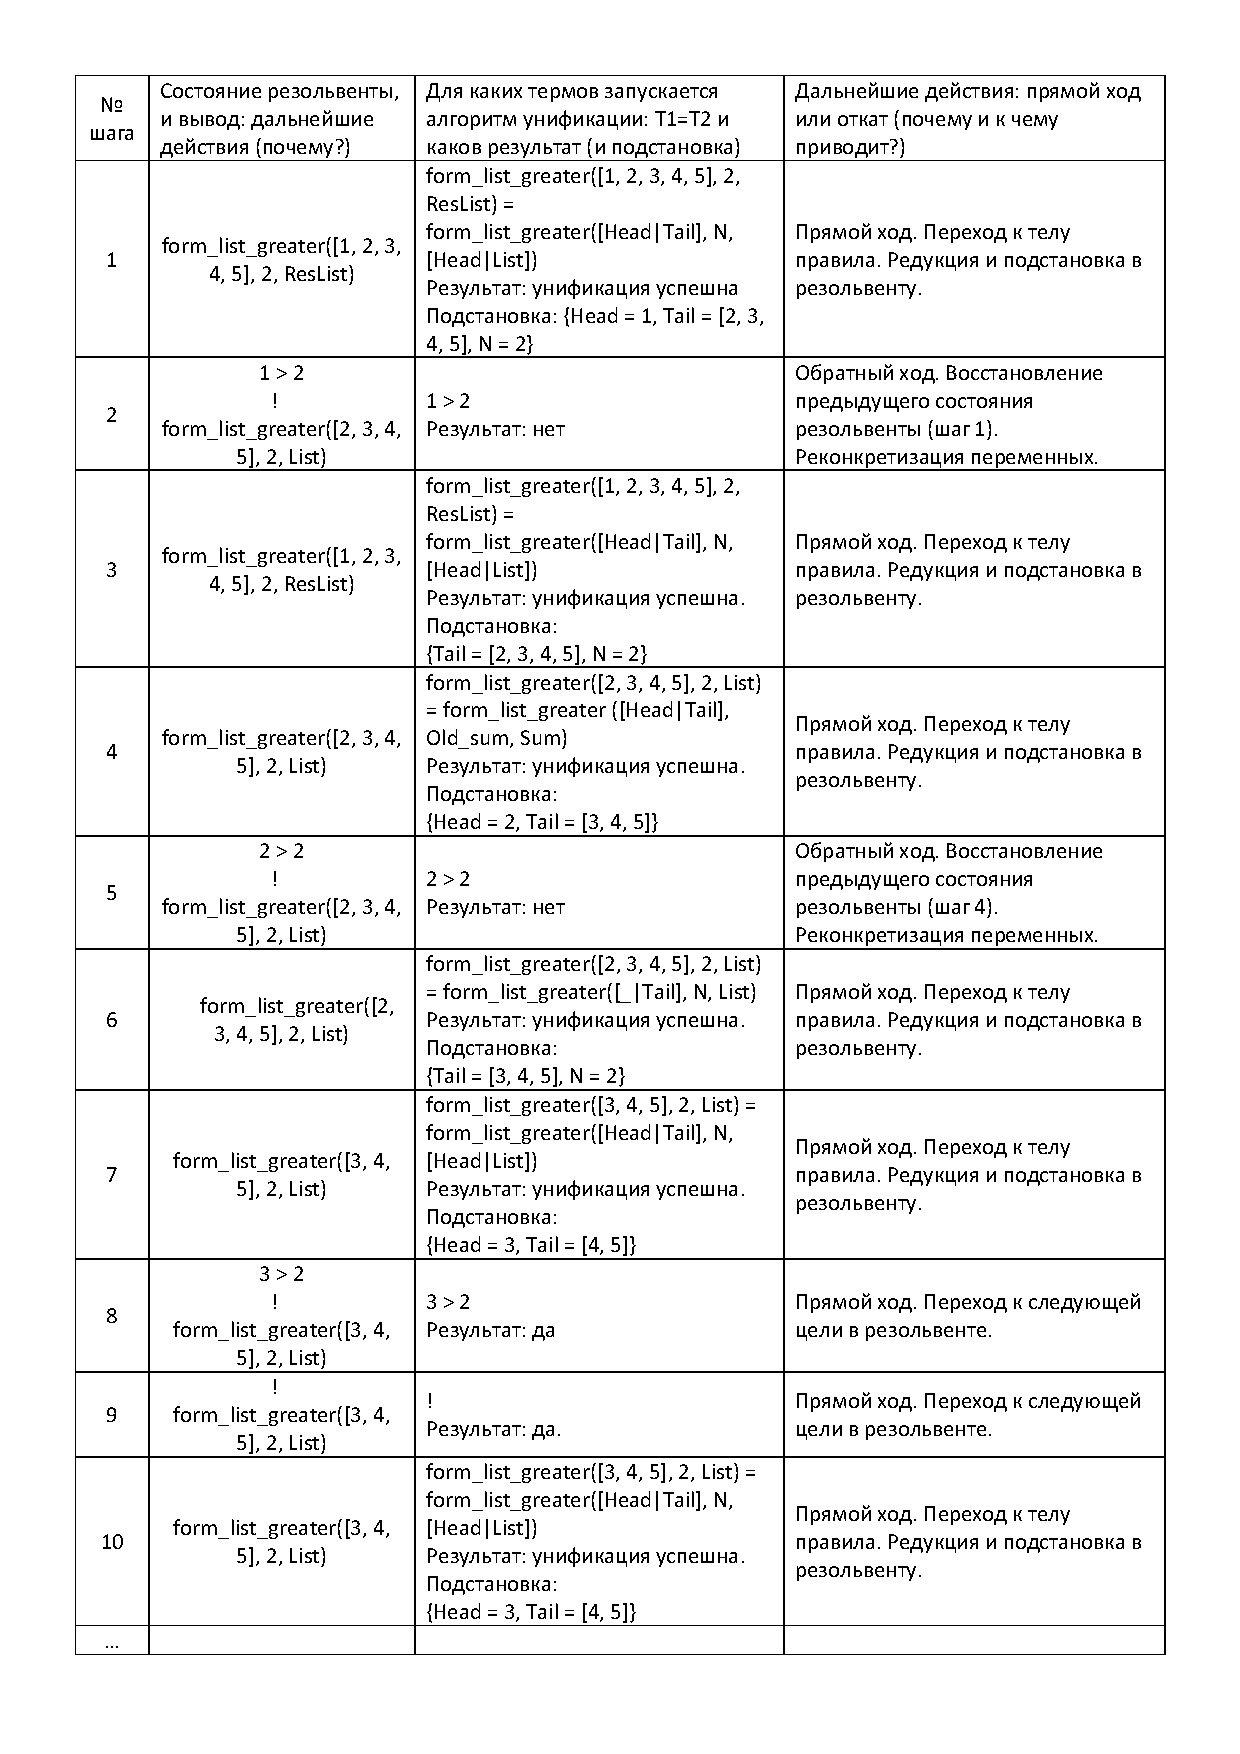
\includegraphics[scale=0.9]{images/table_8_1.pdf}
		\caption{Таблица порядка поиска ответов для нахождения суммы элементов списка.}
		\label{image:table_1}
	}
\end{figure}

\begin{figure}[H]
	\centering{
		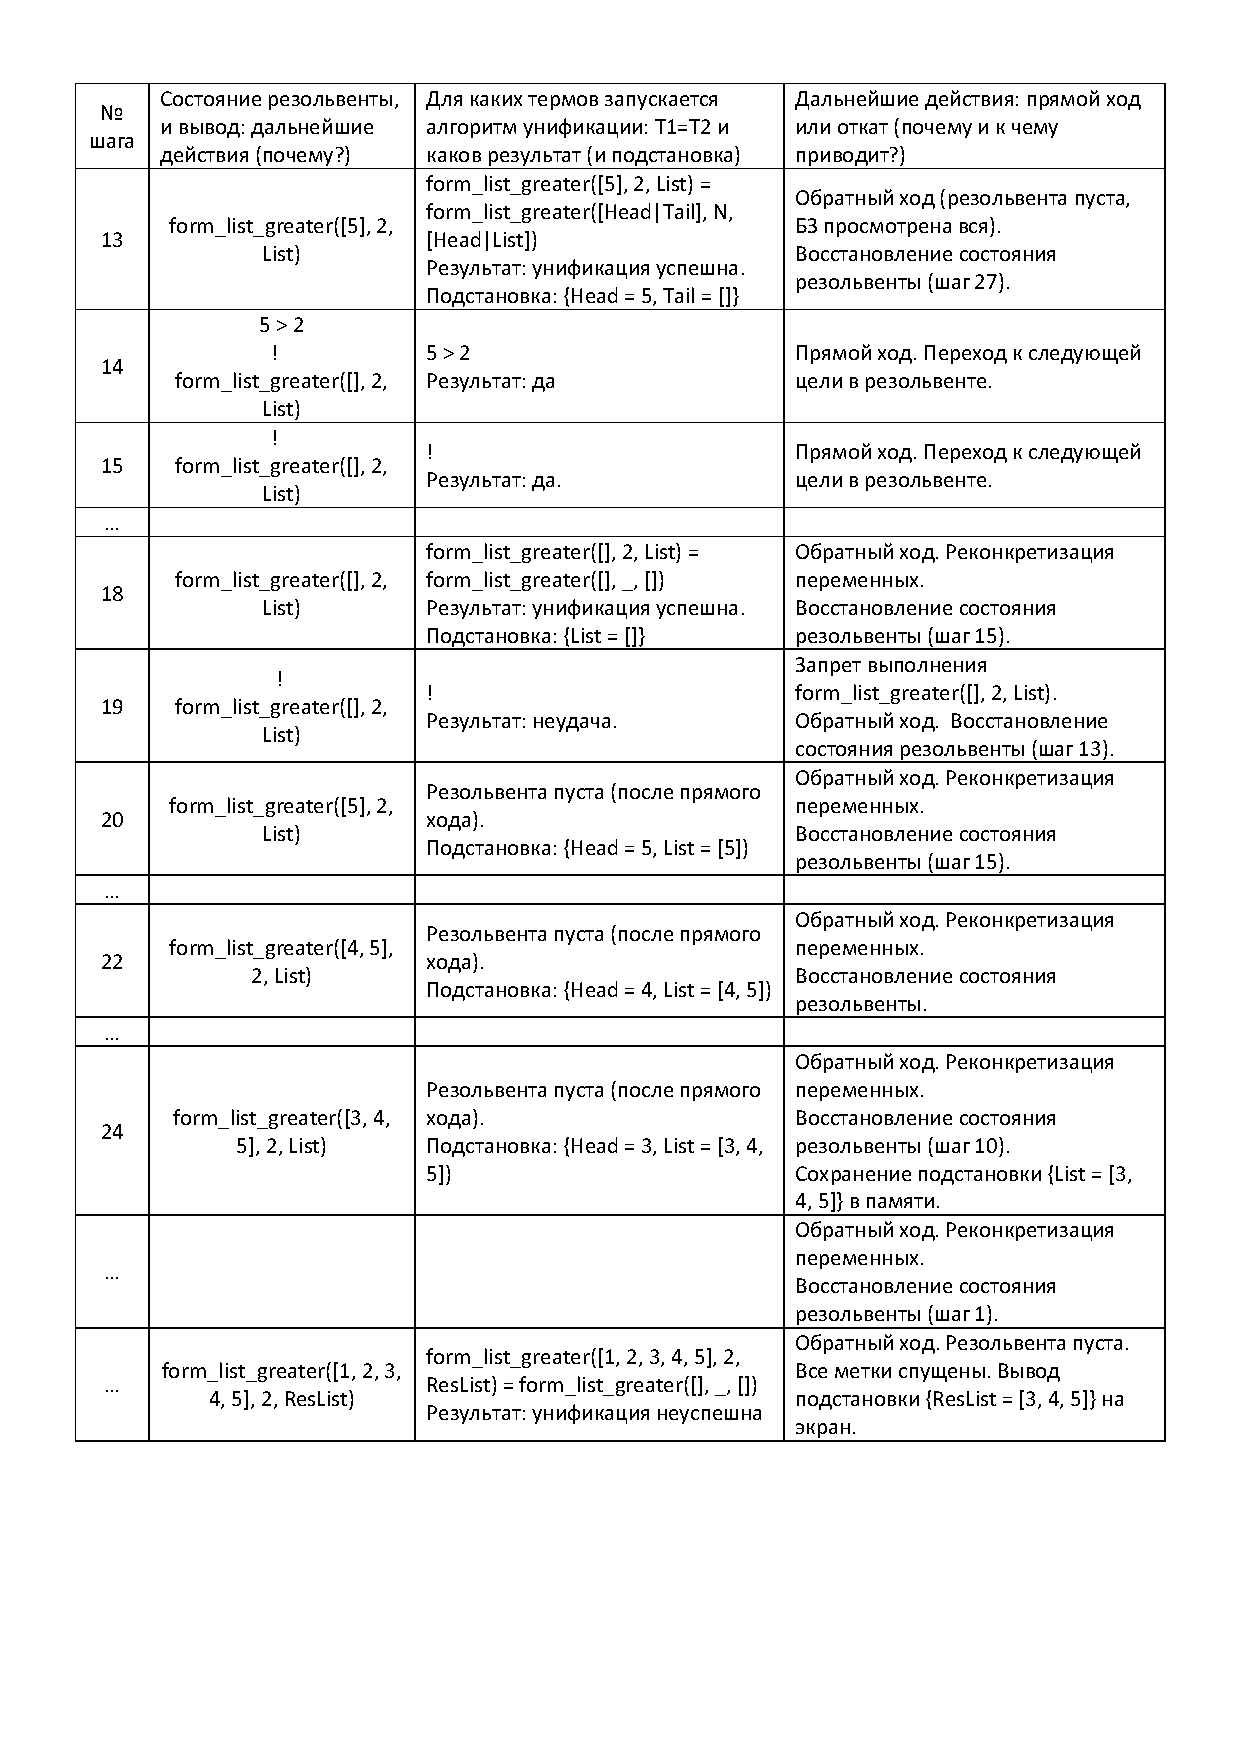
\includegraphics[scale=0.9]{images/table_8_2.pdf}
		\caption{Таблица порядка поиска ответов для нахождения суммы элементов списка (продолжение).}
		\label{image:table_2}
	}
\end{figure}